\chapter{Results}

% \todo[inline]{
%     how you collected and analysed your data – you only need to include enough detail that another expert in the field could repeat what you've done (you don't have to detail field standard techniques or tests) \\
%         - simulation \\
%         - prism model \\
%         - state diagram generator \\
%     why you chose to collect specific data \\
%     how this data will help you to answer your research questions \\
%     why you chose the approach you went with. \\
% }

% \todo[inline]{
%     specify the data you collected and how it was were prepared for analysis \\
%     describe the data analysis (e.g. define the type of statistical test that was applied to the data) \\
%     describe the outcome of the analysis \\
%     present a summary and descriptive statistics in a table or graph.
% }

All experimentation was done on the system detailed in \cref{appendix:computerspecs} using the implementations defined in the previous sections. The repository containing all source code is at \url{https://gitlab.com/harberger-tax} and is freely accessible should it be of use to anyone.

\section{PRISM-games} \label{section:prism-results}

\subsection{Implementation}

The implemented model can be found in \cref{appendix:prism-model} or on Gitlab \footnote{https://gitlab.com/harberger-tax/prism-models}. It is written as a concurrent stochastic game (\texttt{csg}) with three players (a pool and two participants) and requires the following parameters: 

\begin{itemize}
    \item $p$ - The probability of player 1 purchasing.
    \item $q$ - The probability of player 2 purchasing.
    \item $tr$ - The tax rate.
    \item $dr$ - The discount rate.
\end{itemize}.

The model is split into two phases per round. First, in the decision phase, all participants make a decision on whether or not to participate and if participating, who to purchase from. Next, in the purchase phase, all purchases are executed. The model was split into two phases in order to prevent double-purchasing where both participant may attempt to purchase from a participant with a single chunk.

In order for PRISM-games to verify the model, rewards were associated with each phase. First, an amortised block reward reduced by tax and discount factor is awarded during the decision phase. Next, a participant is rewarded or penalised during the purchase phase if they bought or sold a chunk.

\subsection{Results}

Attempting to build the PRISM-games model more than 120 steps resulted in an unknown error, most likely due to being unable to acquire the necessary memory required, or being unable to support the required number of states. Additionally, there was no easy way to programmatically test with different parameters. Hence, PRISM-games was discarded in favour of a custom implementation with the deterministic state generator.


\section{Deterministic State Generator}

\subsection{Methodology}

As the hardware limitations prevent the creation of complete system models, a smaller subset was utilised for analysis. All systems were created with the following parameters (parameters were inflated to accelerate the decay of reward valuation):

\begin{itemize}
    \item Blockchain 
    \begin{itemize}
        \item Block reward - 1
    \end{itemize}  
    \item Pool 
    \begin{itemize}
        \item Initial chunks - 2
    \end{itemize}
    \item Participants
    \begin{itemize}
        \item Initial funds - 1
        \item Initial chunks - 0
    \end{itemize}
    \item Reward minimum threshold - 0.009
    \item Maximum depth - 15
\end{itemize}

The following metrics were recorded regarding each participants potential expected reward based on different participation chances.

\begin{itemize}
    \item The most equal state (smallest difference in balance).
    \item The least equal state (greatest difference in balance).
    \item Total end states.
    \item Total end states within the given wealth-difference.
    \item Metrics for each participant which includes:
    \begin{itemize}
        \item The number of states reachable with the highest balance.
        \item The highest balance possible.
        \item The number of states reachable with the lowest balance.
        \item The lowest balance possible.
        \item The total number of states within the given wealth-difference.
    \end{itemize}
\end{itemize}

\subsection{Results}

Even before generating any states, some intuitive assumptions can be made regarding the potential outcomes of a game in which only two participants exist:

\begin{itemize}
    \item If both participants purchase from the pool in the first step and continue to purchase from each other or do not purchase at all in consequent steps, they will always be in  equilibrium (i.e. equal balance).
    \item The highest possible balance achievable while in equilibrium is if both participants hold a chunk each and do not purchase.
    \item The results will be symmetric for participants (unless probability or initial state is different).
\end{itemize}

Consider a game in which the initial state is as follows.

\begin{itemize}
    \item Pool - chunks: 2, balance: 0
    \item Participant 1 - chunks: 0, balance: 1
    \item Participant 2 - chunks: 0, balance: 1
\end{itemize}

The expected payout for all action combinations can be seen in \cref{table:payout1} below. 

\begin{table}[H]
  \centering
  \caption{Expected payout for a basic two-player game}
  \label{table:payout1}
  \begin{tabular}{|l||*{5}{c|}}\hline
    \backslashbox{Participant 1}{Participant 2} & \makebox{Skip} & \makebox{Purchase} \\
    \hline \hline
    Skip                                        & 0, 0           & 0, 1 \\ \hline
    Purchase                                    & 1, 0           & 2, 2 \\ \hline
  \end{tabular}
\end{table}

In the case where both participants skip (Skip, Skip), they receive no rewards (having no chunks). If both participants purchase at the same time (Purchase, Purchase), they expend their balance in order to buy the chunk from their opponent and receive an equal amount of funds for selling their chunk to their opponent, resulting in no net change in balance. Then, during the reward phase, both participants receive one unit for having one chunk in their possession. In cases where only one participant purchases (Skip, Purchase), only the purchaser expends their balance but does not receive any as a chunk was not purchased from them. Next, they receive a reward, restoring their balance back to 1. In this case, the participant who opted to skip would consider purchasing a chunk to catch up, returning to the action combination (Purchase, Purchase). Hence, there exists a Nash equilibrium with the action combination (Purchase, Purchase).

A test was run using the generator for participant probabilities ranging from 0.1 to 0.9 for both participants with a tax rate of 0 and 0.2 (the test script can be found in \cref{appendix:testparticipationprobability}). Only one participant is considered as they are symmetrical in all aspects.

\begin{figure}[H]
  \centering
  \caption{Expected reward per combination of participant purchase probability}
  \label{figure:state-expected}
  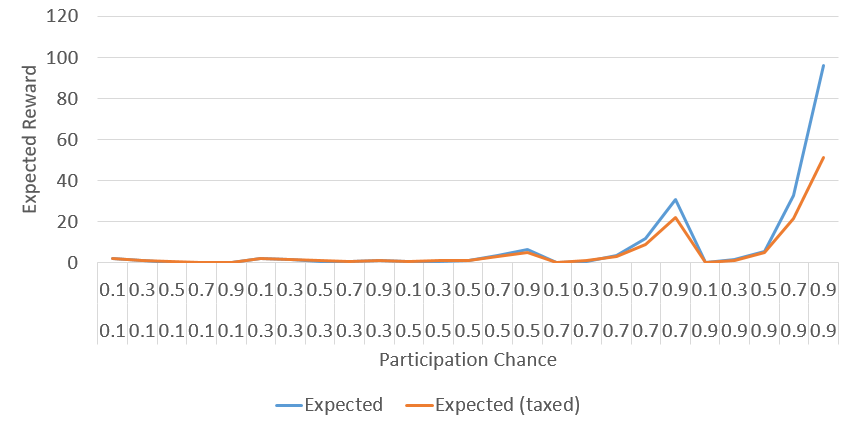
\includegraphics[width=\textwidth]{media/state-expected.PNG}
\end{figure}

The results seen in \cref{figure:state-expected} above shows the expected reward per combination of participation chances. Participant 1 on the bottom row and participant 2 on the top row. It can be observed that higher participation rates yield a higher expected reward, with spikes each time both participation chances reach a relatively high value. This is likely due to the fact that as the product of the probabilities yields the maximum possible chance a state may achieve, reducing the expected reward accordingly. For example, given participants 1 and 2 both have a 0.1 chance to participate, the combination is $0.1 \times 0.1 = 0.01$, meaning the final reward is reduced by x100. Similarly, given participants 1 and 2 both have 0.9 chance to participate, the combination $0.9 \times 0.9 = 0.81$ is significantly higher with at most a 19\% reduction. It is also noted that the impact of the tax becomes more pronounced as the probability to purchase increases. This is likely due to participants being taxed more frequently as they are more likely to possess chunks given the higher purchase probability.

Figure \ref{figure:state-bestworst} below shows the probability of reaching the states with the highest and lowest balance.

\begin{figure}[H]
  \centering
  \caption{Probability of reaching state with highest and lowest balance}
  \label{figure:state-bestworst}
  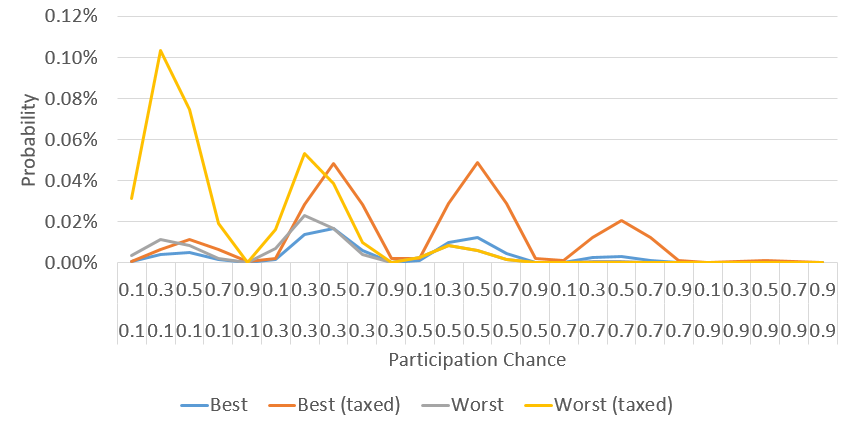
\includegraphics[width=\textwidth]{media/state-bestworst.PNG}
\end{figure}

The peaks in the worst (taxed) trend-line may be due to the low purchase likelihood of the participant directly benefiting the other participant, leading the the largest difference in funds. This was predicted in \cref{table:payout1} in the action combinations (Skip, Purchase). As the purchase probability increases, the peaks reduce in magnitude as probability to reach an equilibrium state increases, decreasing the probability to reach a worst case state. Similarly, the best states are only achievable if neither participant is especially inclined to purchase, increasing the probability of traversing a chain of transitions in which one participant does not purchase chunks, letting the other participant accumulate the rewards unchecked.

Figure \ref{figure:state-expected-tax} below shows the expected reward as tax increases. The test script can be found in \cref{appendix:testparticipationtax} and the raw data can be found in \cref{appendix:state-results-tax} As expected, the reward decreases in a linear fashion as the tax increases.

\begin{figure}[H]
  \centering
  \caption{Expected reward per tax rate}
  \label{figure:state-expected-tax}
  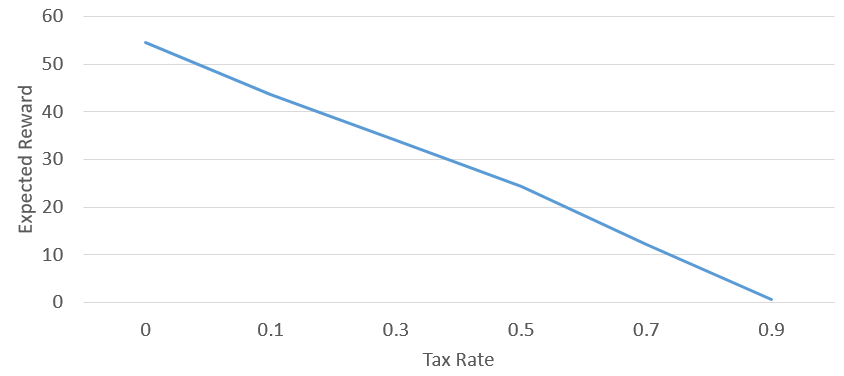
\includegraphics[width=\textwidth]{media/state-expected-tax.PNG}
\end{figure}


\section{Simulation}

\subsection{Methodology}

As the simulation is not limited by hardware, all executions are able to run to completion. All simulations were run with the following parameters (similarly exaggerated to accelerate decay):

\begin{itemize}
    \item Blockchain
    \begin{itemize}
        \item Block reward - 12.5
        \item Global hash rate - 1
        \item Block time - 1
        \item Discount factor - 0.001\%
    \end{itemize}
    \item Pool 
    \begin{itemize}
        \item Hash rate - 0.3 (i.e. 30\%)
        \item Tax rate - 5\%
        \item Trade interval - 0.5
    \end{itemize}
    \item Participants
    \begin{itemize}
        \item Count - 3
        \item Initial chunks - 0
    \end{itemize}
    \item Reward minimum threshold - 0.009
\end{itemize}

\subsection{Results}

Figures \ref{figure:simulation-balance} and \ref{figure:simulation-chunks} are the results of a simulation with three participants, four chunks, and limited to 200 rounds. Figure \ref{figure:simulation-balance} below shows that the general trend is fairly balanced in the beginning but begins to diverge as balances increase. While participant 3 lags behind, this can be explained by the their reduced activity as seen in \cref{figure:simulation-chunks}. Despite this, the average distribution of funds observe a positive trend given the right conditions and do not diverge significantly.

\begin{figure}[H]
  \centering
  \caption{Balance distribution over shortened simulation lifespan}
  \label{figure:simulation-balance}
  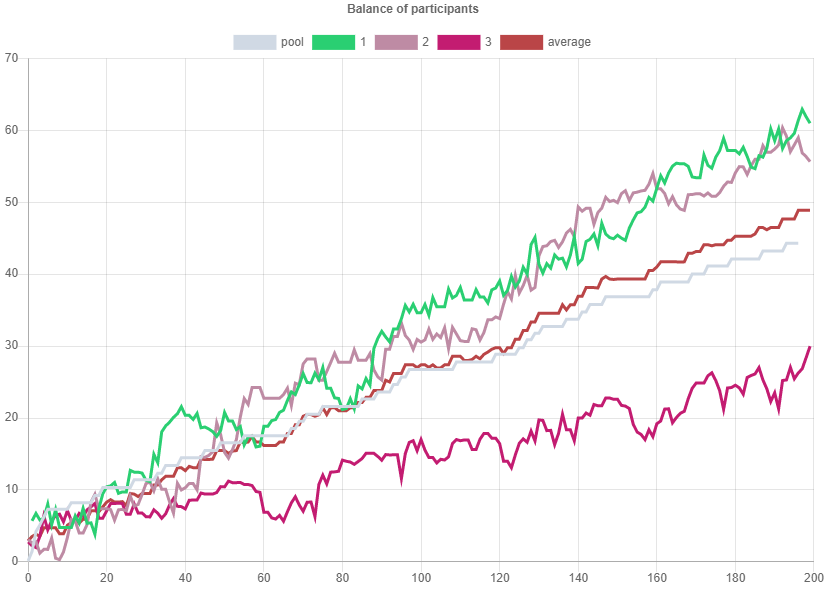
\includegraphics[width=0.8\textwidth]{media/simulation-balance.PNG}
\end{figure}

As seen in \cref{figure:simulation-chunks} below, the transition of funds occurred fairly frequently, effectively reducing any chance a participant may have in holding all the chunks. It is noted that there were several instances when a participant was able to hold all the chunks. while they were never in a participants possession for longer than a single round, it is less than ideal as it is possible for the game to reach such a state. Despite these spikes, the balances did not experience any sudden jumps in correlation to the possession of all chunks. This is likely due to the trade interval being half that of the block time, meaning a participant will likely have to maintain possession of the chunk for two rounds. 

\begin{figure}[H]
  \centering
  \caption{Chunk distribution over shortened simulation lifespan}
  \label{figure:simulation-chunks}
  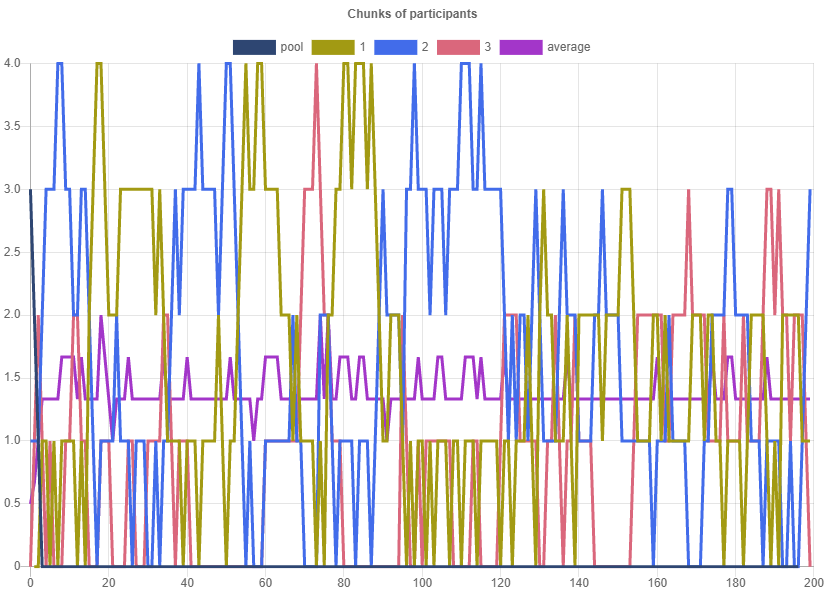
\includegraphics[width=0.8\textwidth]{media/simulation-chunks.PNG}
\end{figure}

Figures \ref{figure:simulation-converge-balance} and \ref{figure:simulation-converge-chunks} are the results of a simulation with three participants, six chunks, and was allowed to run to completion (based on the discount factor and reward threshold). Figure \ref{figure:simulation-converge-balance} shows an ideal situation in which despite varying degrees of growth, the final trend is towards the average. It shows that as participants purchase from one another, they may still have chunks in reserve, accumulating rewards passively as they trade as they are able to consistently maintain ownership of chunks for longer. In this case, the balance is likely to converge despite differing participation probabilities as participants effectively inhibit divergence through consistent trading. It is noted that the number of rounds is less than the previous simulation. This is due to the increased number of chunks resulting in lower rewards per chunk as previously defined by \cref{equation:chunkreward}.

\begin{figure}[H]
  \centering
  \caption{Balance distribution over simulation lifespan with increased chunks}
  \label{figure:simulation-converge-balance}
  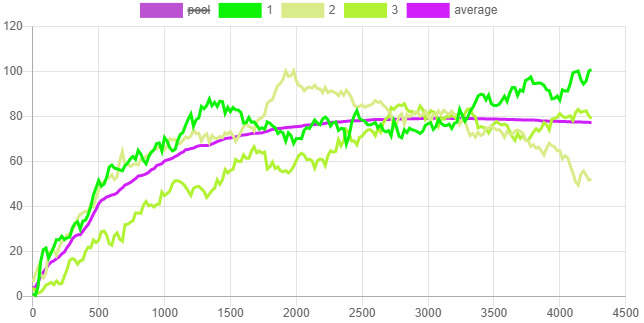
\includegraphics[width=0.8\textwidth]{media/simulation-converge-balance.PNG}
\end{figure}

Figure \ref{figure:simulation-converge-chunks} below shows the maximum difference in chunks held over the lifespan of the simulation. Over the course of the simulation, no participant held more all available chunks for longer than one round, reducing the likelihood of earning the whole balance awarded to the pool.

\begin{figure}[H]
  \centering
  \caption{Averaged chunk distribution over simulation lifespan with increased chunks}
  \label{figure:simulation-converge-chunks}
  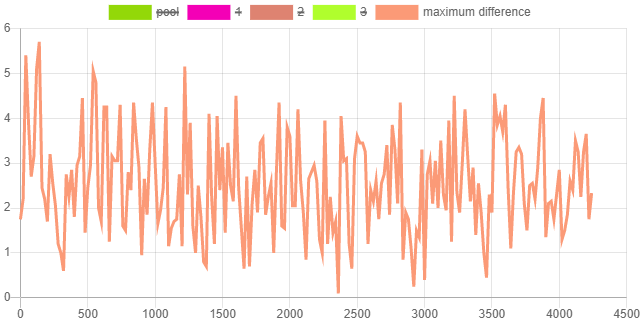
\includegraphics[width=0.8\textwidth]{media/simulation-converge-chunks.PNG}
\end{figure}

Figures \ref{figure:simulation-divergence-balance} and \ref{figure:simulation-divergence-chunks} are the results of a simulation with three participants, two chunks, and was allowed to run to completion (based on the discount factor and reward threshold). As seen in \cref{figure:simulation-divergence-balance} below, the funds appear to diverge as time goes on with one participant reaching close to an no funds. This is likely due to the fact that as the number of chunks is not enough to satisfy all participants, some participants are not able to receive a reward during some rounds and become disadvantaged due to the difference. 

\begin{figure}[H]
  \centering
  \caption{Balance distribution over simulation lifespan with decreased chunks}
  \label{figure:simulation-divergence-balance}
  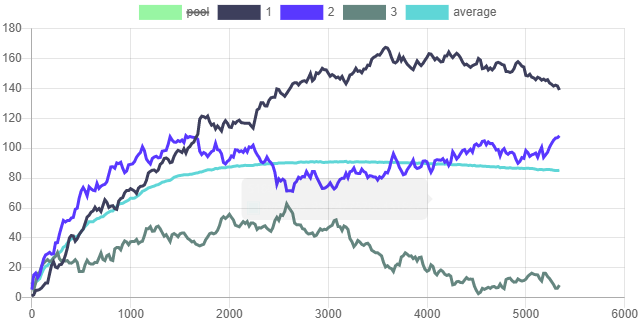
\includegraphics[width=0.8\textwidth]{media/simulation-divergence-balance.PNG}
\end{figure}

Figure \ref{figure:simulation-divergence-chunks} below shows how participant 1 was able to purchase chunks first and immediately gained an advantage with a much higher average chunk count ($\sim$0.9). Meanwhile participant 3 was had a much lower average ($\sim$0.3), leading to much slower growth. This is the least ideal instance of a game as there is a participant with a disproportionate number of chunks and is able to maintain their advantage fairly effectively.
 
\begin{figure}[H]
  \centering
  \caption{Comparison of chunk possession by participant 1 and 3 over simulation lifespan with decreased chunks}
  \label{figure:simulation-divergence-chunks}
  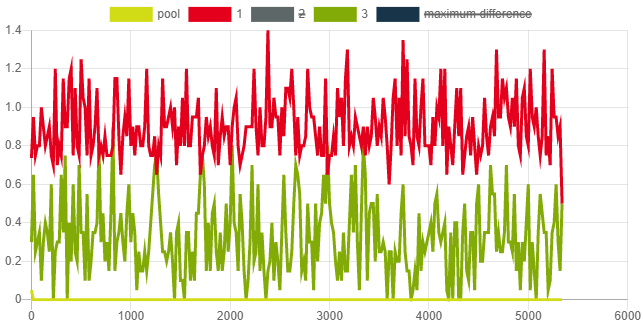
\includegraphics[width=0.8\textwidth]{media/simulation-divergence-chunks.PNG}
\end{figure}

In general, it can be seen that the ratio of chunks to participants may play a significant role in balancing the ease of achieving equilibrium. Despite the possibilities of significant losses, it is also possible to achieve a fairly distributed game if there exists the opportunity for participants to maintain possession of chunks across rounds.

\section{Demonstration} \label{section:demonstration}

A live example demonstrating a simple interactive game with a pool and two participants can be found live on \url{https://harberger-tax.netlify.app/} (as of Nov 1 2020) or in source code on Gitlab \footnote{\url{https://gitlab.com/harberger-tax/demonstration}}. As seen in \cref{figure:demonstration-start} below, the initial funds, chunks, and participation chance can be customised for each participant.

\begin{figure}[H]
  \centering
  \caption{Demonstration initialisation screen}
  \label{figure:demonstration-start}
  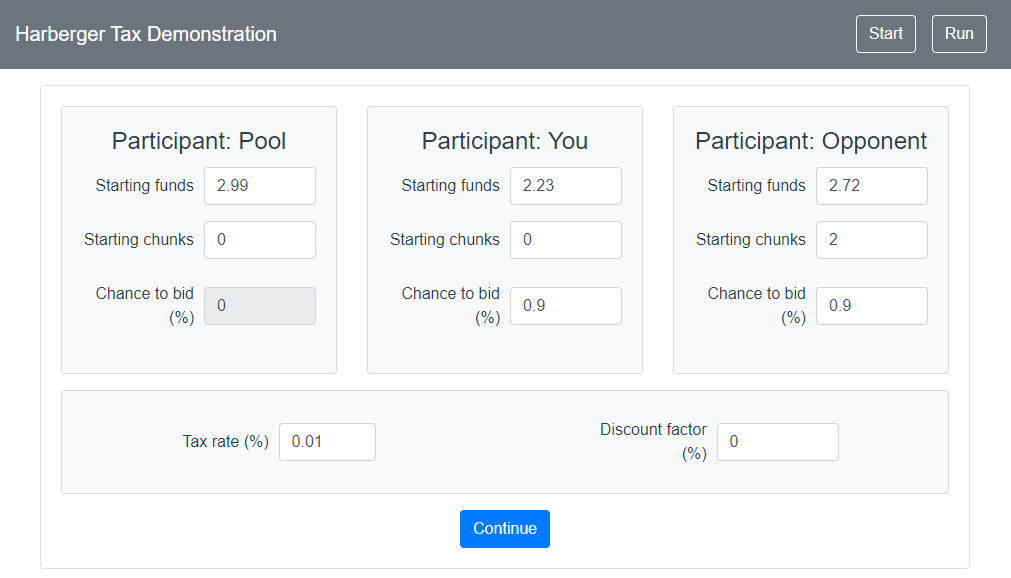
\includegraphics[width=\textwidth]{media/demonstration-start.PNG}
\end{figure}

As seen in \cref{figure:demonstration-run} below, the user is then able to initiate an auction (balance permitting), skip, the round, or let the action be determined randomly during their turn. During the opponents turn, the user may chose to particpate and make a bid or skip. The deterministic state generator has also been integrated to give the user a limited prediction of the game's possible outcomes in the near future.

\begin{figure}[H]
  \centering
  \caption{Demonstration run screen}
  \label{figure:demonstration-run}
  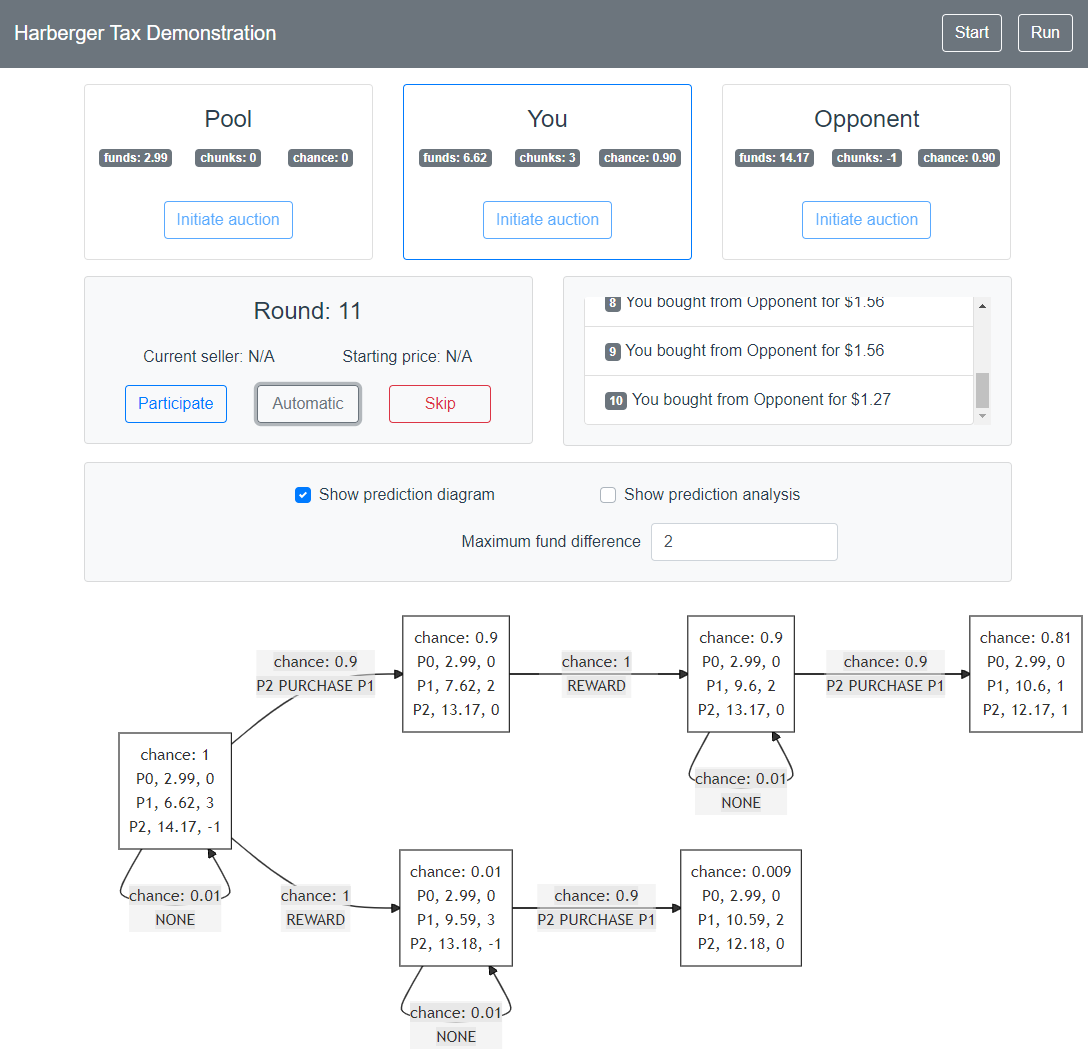
\includegraphics[width=\textwidth]{media/demonstration-run.PNG}
\end{figure}
